\begin{figure}[p]
\centering
\captionsetup{justification=raggedright,labelsep=none,singlelinecheck=false,labelformat=boldlabel}
\caption[]{\footnotesize \textbf{: Predictor-theme loading shares over time for the Market portfolio estimation.} The figure reports descriptive loadings from linear surrogate models. Columns report HAR, HARX, elastic net, random forest, XGBoost, and the three neural-network architectures. The intercept is excluded. Each coefficient is divided by the sum of absolute non-intercept coefficients. Gross shares sum absolute loadings within themes. Net shares retain coefficient signs. Own-series terms refer to each factor's realized measures. The equal-weighted forecast has no fitted surrogate model.}
\label{fig:rv-theme_history_spx}
\par\smallskip\textbf{Panel A. Long sample}\par\smallskip
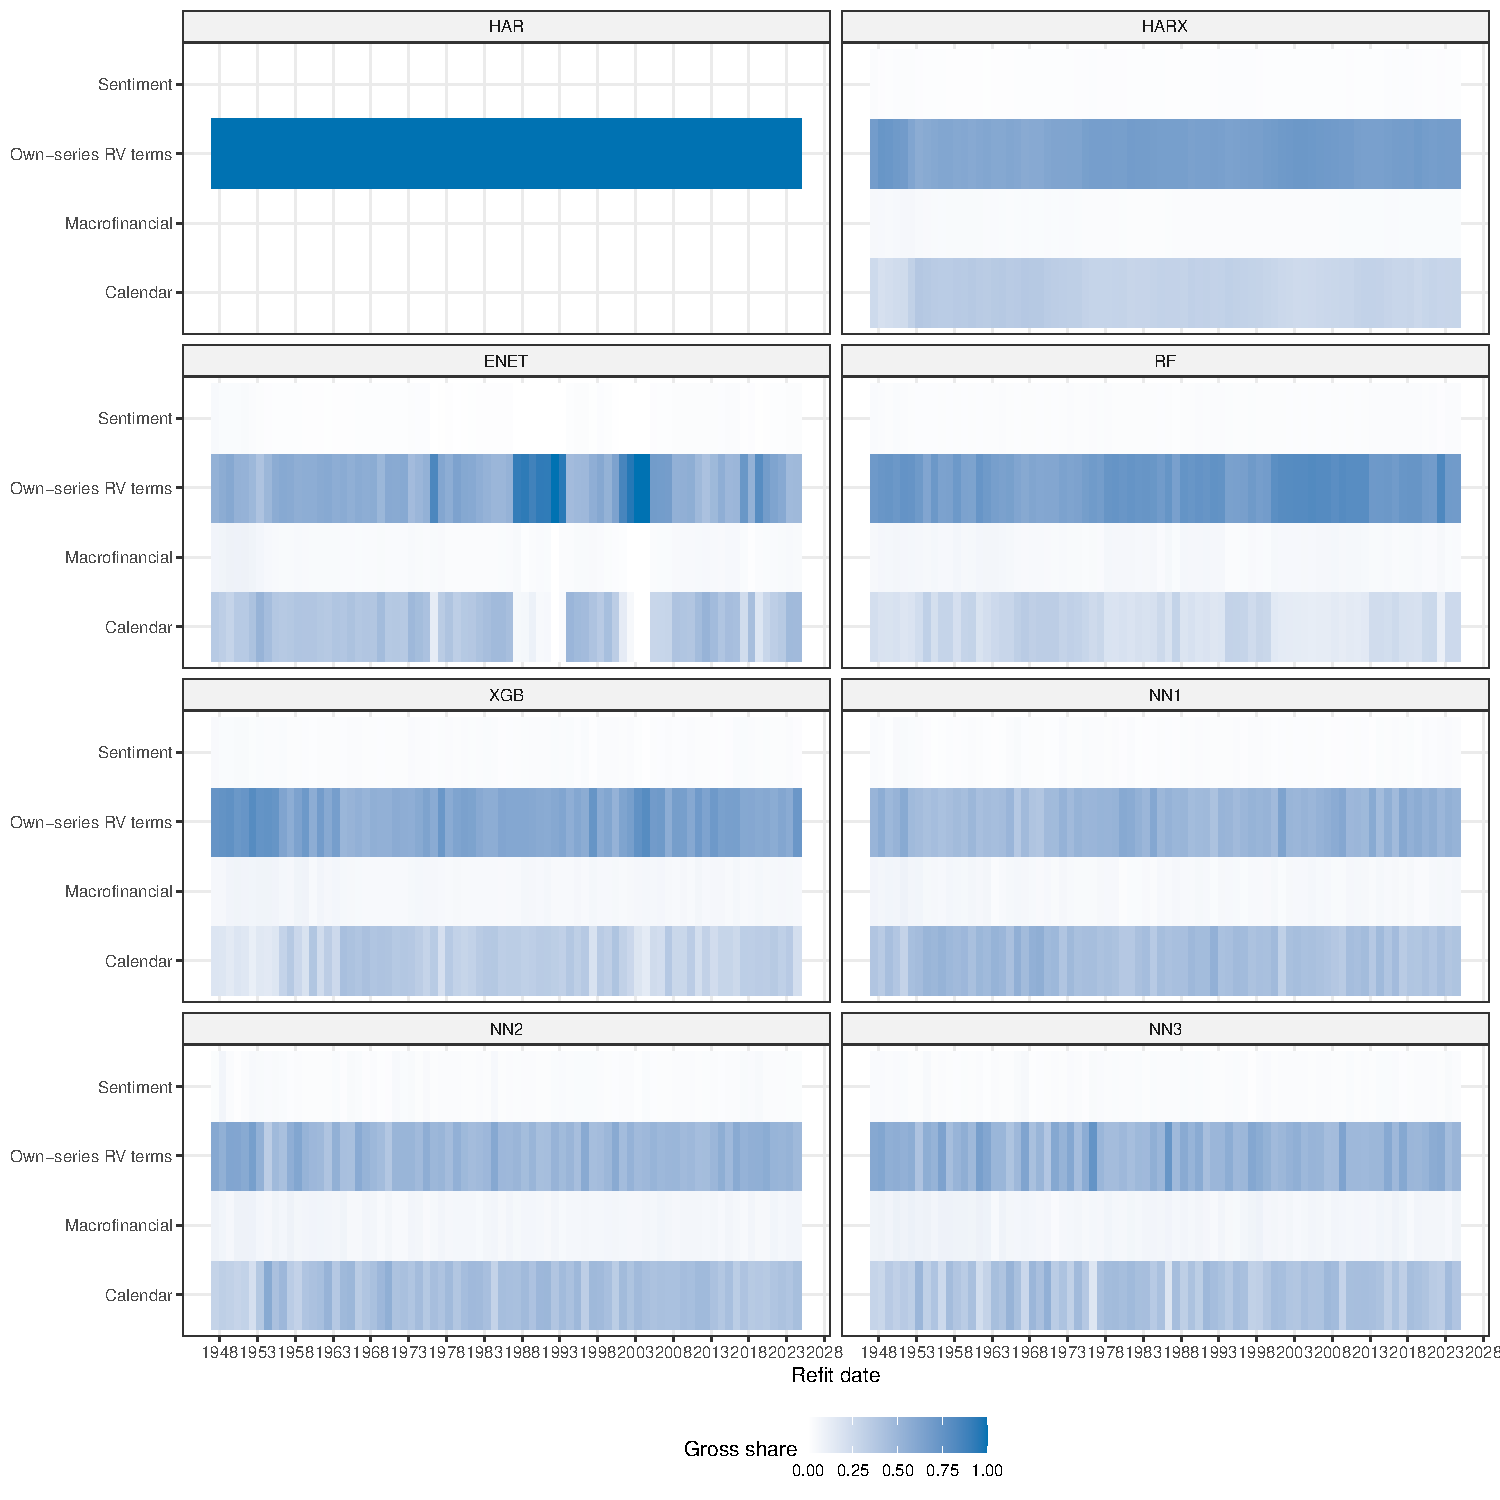
\includegraphics[width=\linewidth,height=0.70\textheight,keepaspectratio]{results_v3/1927/internet_appendix/theme_history_spx.pdf}
\end{figure}
\begin{figure}[p]
\ContinuedFloat
\centering
\captionsetup{justification=raggedright,labelsep=none,singlelinecheck=false,labelformat=boldlabel}
\caption[]{\footnotesize \textbf{: Predictor-theme loading shares over time for the Market portfolio estimation.} The figure reports descriptive loadings from linear surrogate models. Columns report HAR, HARX, elastic net, random forest, XGBoost, and the three neural-network architectures. The intercept is excluded. Each coefficient is divided by the sum of absolute non-intercept coefficients. Gross shares sum absolute loadings within themes. Net shares retain coefficient signs. Own-series terms refer to each factor's realized measures. The equal-weighted forecast has no fitted surrogate model. Continued.}
\par\smallskip\textbf{Panel B. Short sample}\par\smallskip
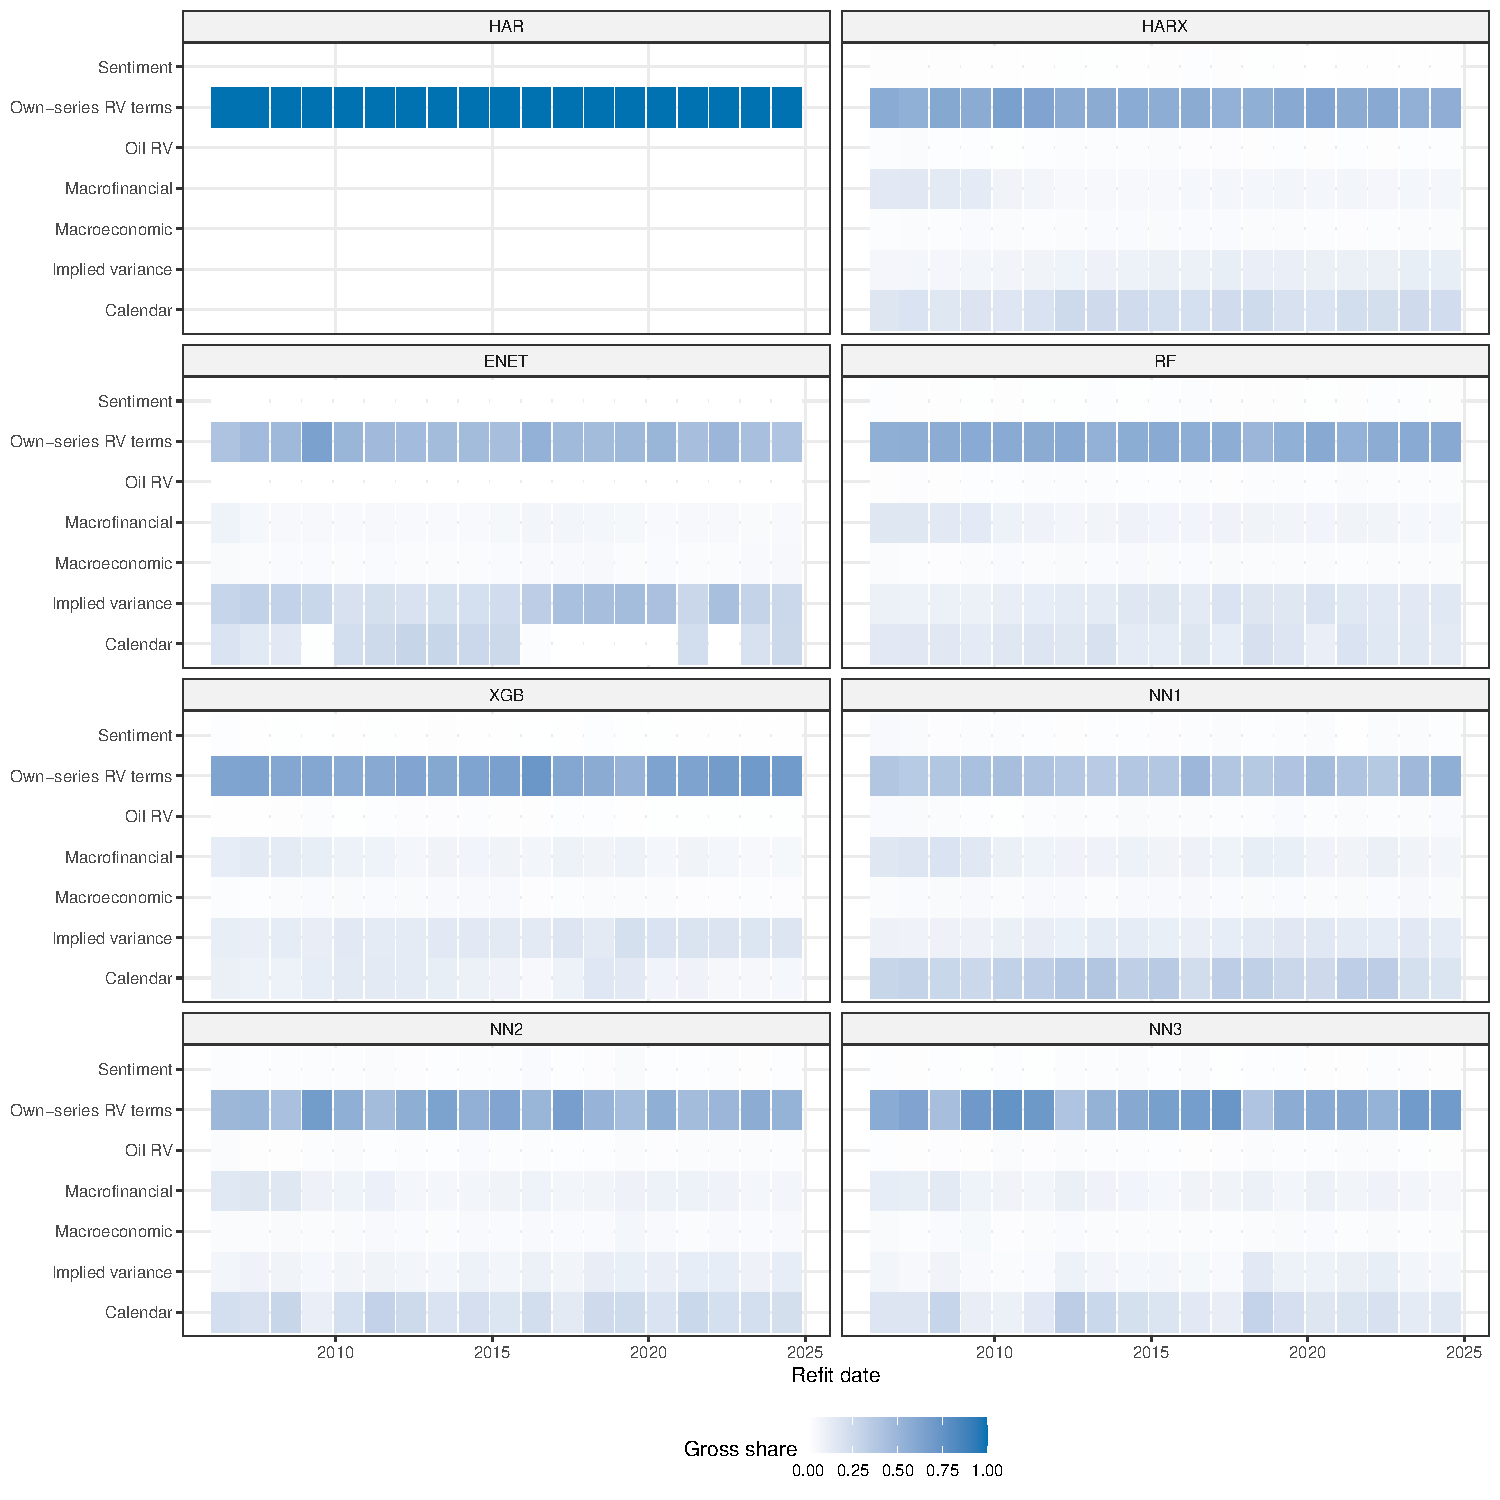
\includegraphics[width=\linewidth,height=0.70\textheight,keepaspectratio]{results_v3/1986/internet_appendix/theme_history_spx.pdf}
\end{figure}
